\documentclass[12pt]{article}
\usepackage[english]{babel}
\usepackage{natbib}
\usepackage{url}
\usepackage[utf8x]{inputenc}
\usepackage{amsmath}
\usepackage{graphicx}
\usepackage{parskip}
\usepackage{fancyhdr}
\usepackage{vmargin}
\usepackage{amssymb}
\usepackage{wasysym}
\usepackage{comment}
\newcommand\floor[1]{\lfloor#1\rfloor}
\newcommand\ceil[1]{\lceil#1\rceil}
\begin{comment}
\usepackage{titlesec}
\titleformat{\subsection}[runin]
  {\normalfont\large\bfseries}{\thesubsection}{1em}{}
\titleformat{\subsubsection}[runin]
  {\normalfont\small}{\thesubsubsection}{1em}{}
\end{comment}  
\setmarginsrb{1.5 cm}{2 cm}{1.5 cm}{2 cm}{1 cm}{1.5 cm}{1 cm}{1.5 cm}

\makeatletter
\newcommand{\rmnum}[1]{\romannumeral #1}
\newcommand{\Rmnum}[1]{\expandafter\@slowromancap\romannumeral #1@}
\makeatother

\title{EE 338 : Filter Design Assignment}								% Title
\author{Dimple Kochar}								% Author
\date{\today}											% Date

\makeatletter
\let\thetitle\@title
\let\theauthor\@author
\let\thedate\@date
\makeatother

\pagestyle{fancy}
\fancyhf{}
\rhead{\theauthor}
\lhead{\thetitle}
\cfoot{\thepage}

\begin{document}

%%%%%%%%%%%%%%%%%%%%%%%%%%%%%%%%%%%%%%%%%%%%%%%%%%%%%%%%%%%%%%%%%%%%%%%%%%%%%%%%%%%%%%%%%

\begin{titlepage}
	\centering
    \vspace*{0.3 cm}
    
\includegraphics[scale = 0.65]{IIT_B_Logo.jpg}\\[1.0 cm]	% University Logo
    \textsc{\Large Indian Institute of Technology, Bombay}\\[2.0 cm]	% University Name
	\textsc{\LARGE Digital Signal Processing}\\[0.5 cm]				% Course Code
	\textsc{\Large EE - 338}\\[0.5 cm]				% Course Name
	\rule{\linewidth}{0.2 mm} \\[0.4 cm]
	{ \huge \bfseries Filter Design Assignment}\\
	\rule{\linewidth}{0.2 mm} \\[1.5 cm]
	
	\begin{minipage}{0.4\textwidth}
		\begin{flushleft} \large
			\emph{Name :}\\
			\theauthor
			\end{flushleft}
			\end{minipage}~
			\begin{minipage}{0.4\textwidth}
			\begin{flushright} \large
			\emph{Roll Number :} \\
			16\textsc{D}070010									% Your Student Number
		\end{flushright}
	\end{minipage}\\[2 cm]
	
	{\large April 11, 2019}\\[2 cm]
 
	\vfill
	
\end{titlepage}

%%%%%%%%%%%%%%%%%%%%%%%%%%%%%%%%%%%%%%%%%%%%%%%%%%%%%%%%%%%%%%%%%%%%%%%%%%%%%%%%%%%%%%%%%

\tableofcontents
\pagebreak

%%%%%%%%%%%%%%%%%%%%%%%%%%%%%%%%%%%%%%%%%%%%%%%%%%%%%%%%%%%%%%%%%%%%%%%%%%%%%%%%%%%%%%%%%

\section{Student Details}
\textbf{Name } \hspace{2 cm}: \textit{Dimple Kochar}\\
\textbf{Roll Number } \hspace{0.5 cm}: \textit{16\textsc{D}070010}\\
\textbf{Filter Number }\hspace{0.2 cm}      : \textsc{79}

\vspace{0.5 cm}
\section{Filter-1(Bandpass) Details}
%--------------------------------------------------------------------------------------------------------------------------
\subsection{Un-normalized Discrete Time Filter Specifications}
Filter Number = 79
\\Since filter number is $>$75 , m = 79 - 75 = 4 and passband will be equiripple\\
q(m) = greatest integer strictly less than 0.1*m = greatest integer strictly less than 0.4 = 0\\
r(m) = m - 10*q(m) = 4 - 10*0 = 4\\
$B_{L}$(m) = 5 + 1.4*q(m) + 4*r(m) = 5 + 1.4*0 + 4*4 = 21\\
$B_{H}$(m) = $B_{L}$(m) + 10 = 21 + 10 = 31\\ 
\\We have to design a \textbf{\textit{Band-Pass}} filter with passband from $B_{L}$(m) kHz to $B_{H}$(m) kHz. Therefore the specifications are as follows: \\
\begin{itemize}
\item \textbf{Passband} : 21 kHz to 31 kHz
\item \textbf{Transition Band} : 2 kHz on either side of passband
\item \textbf{Stopband} : 0-19 kHz and 33-160 kHz\hspace{1.5 cm} ($\because$ Sampling rate is 320 kHz)
\item \textbf{Tolerance} : 0.15 in magnitude for both Passband and Stopband
\item \textbf{Passband Nature} : Equiripple
\item \textbf{Stopband Nature} : Monotonic
\end{itemize}
%--------------------------------------------------------------------------------------------------------------------------
\subsection{Normalized Digital Filter Specifications}
Sampling Rate = 320 kHz\\
Any frequency($\Omega$) upto 160 kHz($\frac{Sampling Rate}{2}$) can be represented on the normalized axis($\omega$) as (since in the normalized frequency axis, sampling rate 
corresponds to 2$\pi$) :\\
\begin{equation*}
\omega = \frac{\Omega*2\pi}{\Omega _{s}(Sampling Rate)}
\end{equation*}

Therefore the corresponding normalized discrete filter specifications are:
\begin{itemize}
\item \textbf{Passband} : 0.13125$\pi$ to 0.19375$\pi$
\item \textbf{Transition Band} : 0.0125$\pi$ on either side of passband
\item \textbf{Stopband} : 0-0.11875$\pi$ and 0.20625$\pi$-$\pi$
\item \textbf{Tolerance} : 0.15 in magnitude for both Passband and Stopband
\item \textbf{Passband Nature} : Equiripple
\item \textbf{Stopband Nature} : Monotonic
\end{itemize}
%--------------------------------------------------------------------------------------------------------------------------
\subsection{Analog filter specifications for Band-pass analog filter using Bilinear Transformation}
The bilinear transformation is given as:
\begin{equation*}
\Omega = tan\left(\frac{\omega}{2}\right)
\end{equation*}
Applying the Bilinear transform to the frequencies at the band-edges, we get:
\begin{table}[h!]
\centering
\begin{tabular}{|l|r|}\hline
$\omega$ & $\Omega$ \\\hline
0 & 0 \\
0.11875$\pi$ & 0.1887 \\
0.13125$\pi$ & 0.2091 \\
0.19375$\pi$ & 0.3141 \\
0.20625$\pi$ & 0.3358 \\
$\pi$ & $\infty$\\ \hline
\end{tabular}
%\caption{\label{tab:widgets}An example table.}
\end{table}

Therefore, the corresponding analog filter specifications using the bilinear transformation are:
\begin{itemize}
\item \textbf{Passband} : 0.2091($\Omega _{P_{1}}$) to 0.3141($\Omega _{P_{2}}$)
\item \textbf{Transition Band} : 0.1887 to 0.2091 \& 0.3141 to 0.3358
\item \textbf{Stopband} : 0 to 0.1887($\Omega _{S_{1}}$) and 0.3358($\Omega _{S_{2}}$) to $\infty$
\item \textbf{Tolerance} : 0.15 in magnitude for both Passband and Stopband
\item \textbf{Passband Nature} : Equiripple
\item \textbf{Stopband Nature} : Monotonic
\end{itemize}
%--------------------------------------------------------------------------------------------------------------------------
\subsection{Frequency Transformation \& Relevant Parameters}
We make use of the Bandpass transformation to transform the Band-Pass analog filter to a Lowpass analog filter. We require two parameters in such a case:\\
\begin{equation*}
\Omega _{L} = \frac{\Omega ^{2} - \Omega _{0}^{2}}{B\Omega}
\end{equation*}
The two parameters in the above equation are B and $\Omega _{0}$. They can be determined using the specifications of the bandpass analog filter using the following relations:\\
\begin{equation*}
\Omega _{0} = \sqrt{\Omega _{P_{1}}\Omega _{P_{2}}} = \sqrt{0.2091 * 0.3141} = 0.2563
\end{equation*}
\begin{equation*}
B = \Omega _{P_{2}} - \Omega _{P_{1}} = 0.3141 - 0.2091 = 0.1050
\end{equation*}
\begin{table}[h!]
\centering
\begin{tabular}{|l|r|}\hline

$\Omega$ & $\Omega_{L}$ \\\hline
$0^{+}$ & -$\infty$ \\
0.1887($\Omega _{S_{1}}$)& -1.5181($\Omega _{L_{S_{1}}}$) \\
0.2091($\Omega _{P_{1}}$)& -1($\Omega _{L_{P_{1}}}$) \\
0.2563($\Omega _{0}$) & 0\\
0.3141($\Omega _{P_{2}}$) & 1($\Omega _{L_{P_{2}}}$) \\
0.3358($\Omega _{S_{2}}$)& 1.3356($\Omega _{L_{S_{2}}}$) \\
$\infty$ & $\infty$\\ \hline
\end{tabular}
%\caption{\label{tab:widgets}An example table.}
\end{table}
%--------------------------------------------------------------------------------------------------------------------------
\subsection{Frequency Transformed Lowpass Analog Filter Specifications}
\begin{itemize}
\item \textbf{Passband Edge} : 1 ($\Omega _{L_{P}}$)  
\item \textbf{Stopband Edge} : min(-$\Omega _{L_{S_{1}}}$,$\Omega _{L_{S_{2}}}$) = min(1.5181, 1.3356) = 1.3356 ($\Omega _{L_{S}}$)
\item \textbf{Tolerance} : 0.15 in magnitude for both Passband and Stopband
\item \textbf{Passband Nature} : Equiripple
\item \textbf{Stopband Nature} : Monotonic
\end{itemize}
%--------------------------------------------------------------------------------------------------------------------------
\subsection{Analog Lowpass Transfer Function}
We need an Analog Filter which has an \textit{equiripple passband} and a \textit{monotonic stopband}. Therefore, we design using the \textbf{Chebyshev} approximation. Since the tolerance($\delta$) in both passband and stopband is 0.15, we define two new quantities in the following way:
\begin{equation*}
D_{1} =  \frac{1}{(1-\delta)^{2}} -1 = \frac{1}{0.85^{2}} -1  = 0.3841
\end{equation*}
\begin{equation*}
D_{2} = \frac{1}{\delta ^{2}} - 1 = \frac{1}{0.15^{2}} - 1 = 43.44
\end{equation*}
\\Now choosing the parameter $\epsilon$ of the Chebyshev filter to be $\sqrt{D_{1}}$, we get the min value of N as:
\begin{equation*}
N_{min} = \ceil{\frac{cosh^{-1}(\sqrt{\frac{D_{2}}{D_{1}}})}{cosh^{-1}(\frac{\Omega _{L_{S}}}{\Omega _{L_{P}}})}}
\end{equation*}
\begin{equation*}
N_{min} = \ceil{3.493} = 4
\end{equation*}
Now, the poles of the transfer function can be obtained by solving the equation:
\begin{equation*}
1 + D_{1}cosh^{2}(N_{min}cosh^{-1}(\frac{s}{j})) = 1 + 0.3841cosh^{2}(4cosh^{-1}(\frac{s}{j})) = 0
\end{equation*}
Solving for the roots (using MATLAB) we get:
\begin{figure}[h!]
	\centering	
	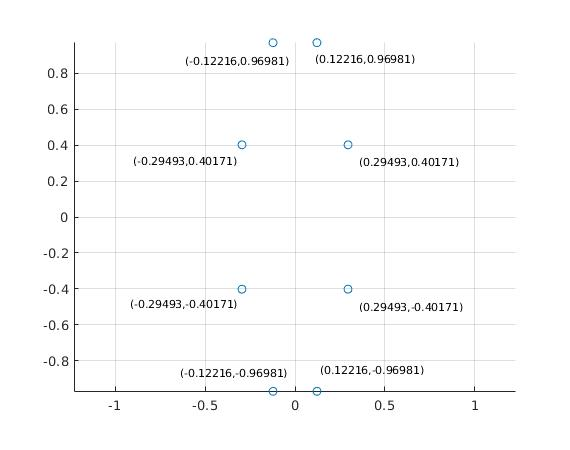
\includegraphics[scale = 0.7]{RootPlot.jpg}
    \caption{Poles of Magnitude Plot of Analog LPF}
\end{figure}
\\Note that the above figure shows the poles of the Magnitude Plot of the Transfer Function. In order to get a stable Analog LPF, we must include the poles lying in the Left Half Plane in the Transfer Function(The poles are symmetric about origin and we can pick one from each pair to be a part of our Transfer Function).
\begin{equation*}
p_{1} = -0.12216 - 0.96981\iota
\end{equation*}
\begin{equation*}
p_{2} = -0.12216 + 0.96981\iota
\end{equation*}
\begin{equation*}
p_{3} = -0.29493 + 0.40171\iota
\end{equation*}
\begin{equation*}
p_{4} = -0.29493 - 0.40171\iota
\end{equation*}

Using the above poles which are in the left half plane and the fact that N is even we can write the Analog Lowpass Transfer Function as:
\begin{equation*}
H_{analog,LPF}(s_{L}) = \frac{(-1)^{4}p_{1}p_{2}p_{3}p_{4}}{\sqrt{(1+D_{1})}(s_{L}-p_{1})(s_{L}-p_{2})(s_{L}-p_{3})(s_{L}-p_{4})}
\end{equation*}
\begin{equation*}
H_{analog,LPF}(s_{L}) = \frac{0.2017}{(s_{L}^{2} + 0.24432s_{L} + 0.95545)(s_{L}^{2} + 0.58984s_{L} + 0.24835)}
\end{equation*}

%--------------------------------------------------------------------------------------------------------------------------
\subsection{Analog Bandpass Transfer Function}
The transformation equation is given by:
\begin{equation*}
s_{L} = \frac{s^{2} + \Omega _{0}^{2}}{Bs}
\end{equation*}
Substituting the values of the parameters B(0.1050) and $\Omega _{0}$(0.2563), we get:
\begin{equation*}
s_{L} = \frac{s^{2} + 0.0657}{0.1050s}
\end{equation*}
\\Substituting this value into $H_{analog,LPF}(s_{L})$ we get $H_{analog,BPF}(s)$ as:
\begin{equation*}
\frac{  0.2448*10^{-4}*s^{4}}{(s^{8}+0.0876s^{7}+0.2776s^{6}+0.0180s^{5}+0.0279s^{4}+0.0012s^{3}+0.0012s^{2}+2.482*10^{-5}s^{1}+1.862*10^{-5})}
\end{equation*}
%--------------------------------------------------------------------------------------------------------------------------
\subsection{Discrete Time Filter Transfer Function}
To transform the analog domain transfer function into the discrete domain, we need to make use of the Bilinear Transformation which is given as:
\begin{equation*}
s = \frac{1-z^{-1}}{1+z^{-1}}
\end{equation*}
Using above equation we get $H_{discrete,BPF}(z)$ from  $H_{analog,BPF}(s)$ as:
\begin{equation*}
\frac{ 10^{-3}*(0.0173-0.0693z^{-2}+0.1039z^{-4}-0.0693z^{-6}+ 0.0173z^{-8})}{1-6.8374z^{-1}+21.3607z^{-2}-39.6324z^{-3}+47.6713z^{-4}-38.0410z^{-5}+19.6800z^{-6}-6.0468z^{-7}+0.8490z^{-8}}
\end{equation*} 
\begin{figure}[h!]
	\centering	
	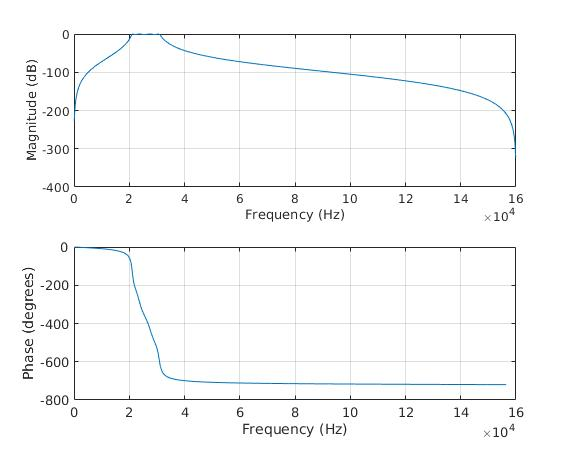
\includegraphics[width = 0.8\textwidth]{matlab_filter1.jpg}
    \caption{Plotting frequency and phase response of filter using freqz command of MATLAB}
\end{figure}
\newpage
%--------------------------------------------------------------------------------------------------------------------------
\subsection{Realization using Direct Form \Rmnum{2}}

\begin{figure}[h!]
	\centering	
	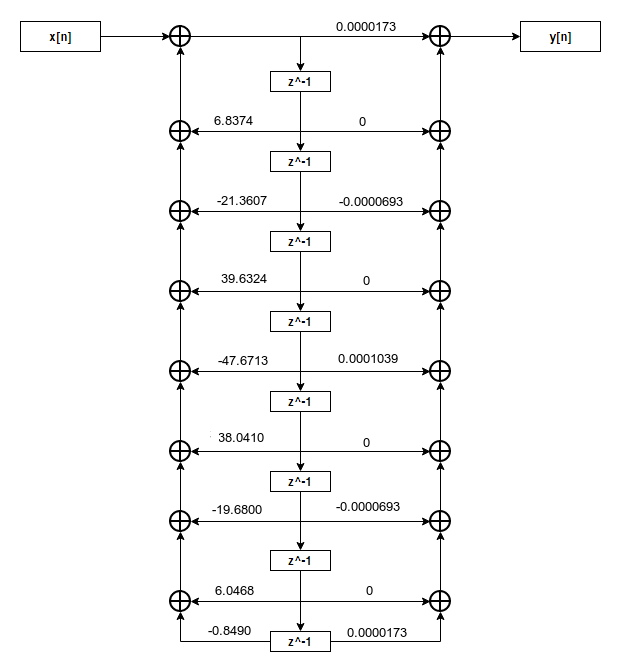
\includegraphics[width = 1\textwidth]{Chebyshev_DirectForm_2.png}
    \caption{Direct Form \Rmnum{2} Block Diagram for $H_{discrete,BPF}(z)$}
\end{figure}

The negative of the denominator coefficients appear as gains on the side of the input sequence x[n] while the numerator coefficients appear on the side of the output y[n] as gains in the signal-flow graph representation of the Direct Form \Rmnum{2}.
%--------------------------------------------------------------------------------------------------------------------------
\subsection{FIR Filter Transfer Function using Kaiser Window}
The tolerance in both the stopband and passband is given to be 0.15.\\
Therefore $\delta$ = 0.15 and we get the  minimum stopband attenuation to be:
\begin{equation*}
A = -20\log (0.15) = 16.4782 dB
\end{equation*}
Since A $<$ 21, we get $\beta$ to be 0 where  $\beta$ is the shape parameter of Kaiser window.\\
Now to estimate the window length required, the lower bound on the window length is found using the empirical formula.
\begin{equation*}
N \geq \frac{A-7.95}{2.285*\Delta\omega _{T}}
\end{equation*}
Here $\Delta\omega _{T}$ is the minimum transition width, which is same on both sides of the passband.
\begin{equation*}
\Delta\omega _{T} = \frac{2 kHz * 2\pi}{320 kHz} =  0.0125\pi
\end{equation*}
\begin{equation*}
\therefore N \geq 95
\end{equation*}
The above equation gives a loose bound on the window length when the tolerance is not very stringent. On successive trials in MATLAB, it was found that a window length of \textbf{131} is required to satisfy the required constraints. \\
\\The time domain coefficients were obtained by first generating the ideal impulse response samples for the same length as that of the window. The Kaiser Window was generated using the MATLAB function and applied on the ideal impulse response samples. The band-pass impulse response samples were generated as the difference between two low-pass filters as done in class.
\newpage
\begin{figure}[h!]
	\centering
    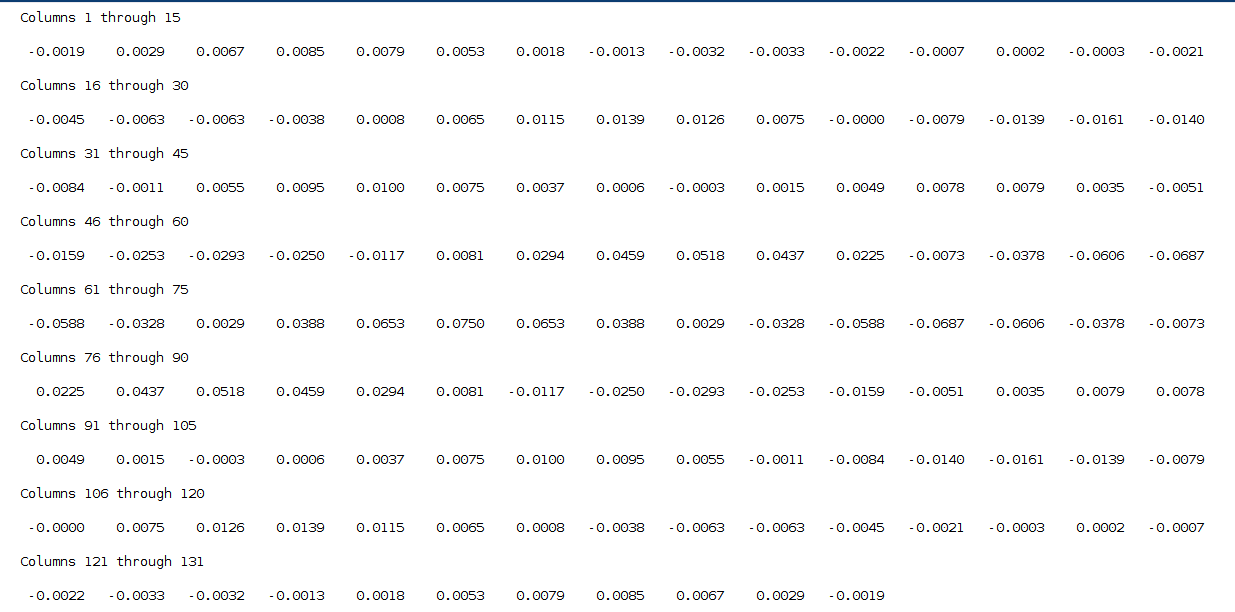
\includegraphics[width = 1\textwidth]{1firt.png}
    \caption{Time domain sequence values}
\end{figure}
\begin{figure}[h!]
	\centering
    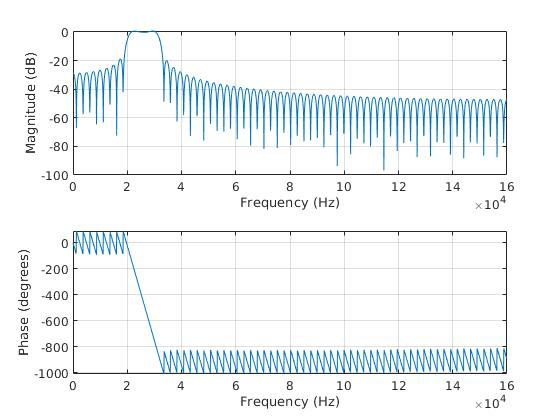
\includegraphics[width = 0.8\textwidth]{1fir.jpg}
    \caption{Plotting frequency and phase response of filter using freqz command of MATLAB}
\end{figure}
The z-transform can simply be read off from the sequence values since its finite sequence.
%--------------------------------------------------------------------------------------------------------------------------
%--------------------------------------------------------------------------------------------------------------------------
%--------------------------------------------------------------------------------------------------------------------------
\newpage
\section{Filter-2(Bandstop) Details}
\subsection{Un-normalized Discrete Time Filter Specifications}
Filter Number = 79
\\Since filter number is $>$75 , m = 79 - 75 = 4 and passband will be monotonic\\
q(m) = greatest integer strictly less than 0.1*m = greatest integer strictly less than 0.4 = 0\\
r(m) = m - 10*q(m) = 4 - 10*0 = 4\\
$B_{L}$(m) = 5 + 1.2*q(m) + 2.5*r(m) = 5 + 1.2*0 + 2.5*4 = 15\\ 
$B_{H}$(m) = $B_{L}$(m) + 6 = 15 + 6 = 21\\ 
\\The second filter is given to be a \textbf{\textit{Band-Stop}} filter with stopband from $B_{L}$(m) kHz to $B_{H}$(m) kHz. Therefore the specifications are:
\begin{itemize}
\item \textbf{Stopband} : 15 kHz to 21 kHz
\item \textbf{Transition Band} : 2 kHz on either side of stopband
\item \textbf{Passband} : 0-13 kHz and 23-125 kHz\hspace{1.5 cm} ($\because$ Sampling rate is 250 kHz)
\item \textbf{Tolerance} : 0.15 in magnitude for both Passband and Stopband
\item \textbf{Passband Nature} : Monotonic
\item \textbf{Stopband Nature} : Monotonic
\end{itemize}
%--------------------------------------------------------------------------------------------------------------------------
\subsection{Normalized Digital Filter Specifications}
Sampling Rate = 250 kHz\\
In the normalized frequency axis, sampling rate corresponds to 2$\pi$ \\
Thus, any frequency($\Omega$) upto 125 kHz($\frac{Sampling Rate}{2}$) can be represented on the normalized axis($\omega$) as:
\begin{equation*}
\omega = \frac{\Omega*2\pi}{\Omega _{s}(Sampling Rate)}
\end{equation*}
Therefore the corresponding normalized discrete filter specifications are:
\begin{itemize}
\item \textbf{Stopband} : 0.12$\pi$ to 0.168$\pi$
\item \textbf{Transition Band} : 0.016$\pi$ on either side of stopband
\item \textbf{Passband} : 0-0.104$\pi$ and 0.184$\pi$-$\pi$
\item \textbf{Tolerance} : 0.15 in magnitude for both Passband and Stopband
\item \textbf{Passband Nature} : Monotonic
\item \textbf{Stopband Nature} : Monotonic
\end{itemize}
%--------------------------------------------------------------------------------------------------------------------------
\subsection{Analog filter specifications for Band-stop analog filter using Bilinear Transformation}
The bilinear transformation is given as:
\begin{equation*}
\Omega = tan\left(\frac{\omega}{2}\right)
\end{equation*}
Applying the Bilinear transform to the frequencies at the band-edges, we get:
\begin{table}[h!]
\centering
\begin{tabular}{|l|r|}\hline
$\omega$ & $\Omega$ \\\hline
0 & 0 \\
0.104$\pi$ & 0.1648 \\             
0.12$\pi$ & 0.1908 \\
0.168$\pi$ & 0.2702  \\
0.184$\pi$ & 0.2974 \\
$\pi$ & $\infty$\\ \hline
\end{tabular}
%\caption{\label{tab:widgets}An example table.}
\end{table}

Therefore the corresponding analog filter specifications for the same type of analog filter using the bilinear transformation are:
\begin{itemize}
\item \textbf{Stopband} : 0.1908($\Omega _{S_{1}}$) to 0.2702($\Omega _{S_{2}}$)
\item \textbf{Transition Band} : 0.1684 to  0.1908 \& 0.2702 to 0.2794
\item \textbf{Passband} : 0 to 0.1684($\Omega _{P_{1}}$) and 0.2974($\Omega _{P_{2}}$) to $\infty$
\item \textbf{Tolerance} : 0.15 in magnitude for both Passband and Stopband
\item \textbf{Passband Nature} : Monotonic
\item \textbf{Stopband Nature} : Monotonic
\end{itemize}
%--------------------------------------------------------------------------------------------------------------------------
\subsection{Frequency Transformation \& Relevant Parameters}
We need to transform a Band-Stop analog filter to a Lowpass analog filter. We require two parameters and can use the bandstop transformation. \\
\begin{equation*}
\Omega _{L} = \frac{B\Omega}{\Omega _{0}^{2} - \Omega^{2}}
\end{equation*}
The two parameters in the above equation are B and $\Omega _{0}$. They can be determined using the specifications of the bandpass analog filter using the following relations:\\
\begin{equation*}
\Omega _{0} = \sqrt{\Omega _{P_{1}}\Omega _{P_{2}}} = \sqrt{0.1648 * 0.2974} = 0.2214
\end{equation*}
\begin{equation*}
B = \Omega _{P_{2}} - \Omega _{P_{1}} = 0.2974 - 0.1648 = 0.1325
\end{equation*}

%Changes required below this
\begin{table}[h!]
\centering
\begin{tabular}{|l|r|}\hline

$\Omega$ & $\Omega_{L}$ \\\hline
$0^{+}$ & $0^{+}$  \\
0.1648($\Omega _{P_{1}}$)& +1($\Omega _{L_{P_{1}}}$) \\
0.1908($\Omega _{S_{1}}$)& +2.0026($\Omega _{L_{S_{1}}}$) \\
0.2214($\Omega _{0}^{-}$) & $\infty$\\
0.2214($\Omega _{0}^{+}$) & -$\infty$\\
0.2702($\Omega _{S_{2}}$) & -1.4924($\Omega _{L_{S_{2}}}$) \\
0.2794($\Omega _{P_{2}}$)& -1($\Omega _{L_{P_{2}}}$) \\
$\infty$ & $0^{-}$ \\\hline
\end{tabular}
%\caption{\label{tab:widgets}An example table.}
\end{table}
%--------------------------------------------------------------------------------------------------------------------------
\subsection{Frequency Transformed Lowpass Analog Filter Specifications}
\begin{itemize}
\item \textbf{Passband Edge} : 1 ($\Omega _{L_{P}}$)  
\item \textbf{Stopband Edge} : min($\Omega _{L_{S_{1}}}$,-$\Omega _{L_{S_{2}}}$) = min(2.0026, 1.4924) = 1.4924 ($\Omega _{L_{S}}$)
\item \textbf{Tolerance} : 0.15 in magnitude for both Passband and Stopband
\item \textbf{Passband Nature} : Monotonic
\item \textbf{Stopband Nature} : Monotonic
\end{itemize}
%--------------------------------------------------------------------------------------------------------------------------
\subsection{Analog Lowpass Transfer Function}
We need an Analog Filter which has a \textit{monotonic passband} and a \textit{monotonic stopband}. Therefore we need to design using the \textbf{Butterworth} approximation. Since the tolerance($\delta$) in both passband and stopband is 0.15, we define two new quantities in the following way:
\begin{equation*}
D_{1} =  \frac{1}{(1-\delta)^{2}} -1 = \frac{1}{0.85^{2}} -1  = 0.3841
\end{equation*}
\begin{equation*}
D_{2} = \frac{1}{\delta ^{2}} - 1 = \frac{1}{0.15^{2}} - 1 = 43.44
\end{equation*}
\\Now using the inequality on the order N of the filter for the Butterworth Approximation we get:
\begin{equation*}
N_{min} = \ceil{\frac{\log{\sqrt{\frac{D_{2}}{D_{1}}}}}{\log{\frac{\Omega_{S}}{\Omega_{P}}}}}
\end{equation*}
\begin{equation*}
N_{min} = \ceil{5.9046} = 6
\end{equation*}
The cut-off frequency($\Omega _{c}$) of the Analog LPF should satisfy the following constraint:
\begin{equation*}
\frac{\Omega_{P}}{D_{1}^{\frac{1}{2N}}} \le \Omega _{c} \le \frac{\Omega_{S}}{D_{2}^{\frac{1}{2N}}}
\end{equation*}
\begin{equation*}
1.083 \le \Omega _{c} \le 1.0899
\end{equation*}
Thus we can choose the value of $\Omega _{c}$ to be 1.085\\
Now, the poles of the transfer function can be obtained by solving the equation:
\begin{equation*}
1 + \left(\frac{s}{j\Omega _{c}}\right)^{2N} = 1 + \left(\frac{s}{j1.085}\right)^{12}  = 0
\end{equation*}
Solving for the roots (using MATLAB) we get:
\begin{figure}[h!]
	\centering	
	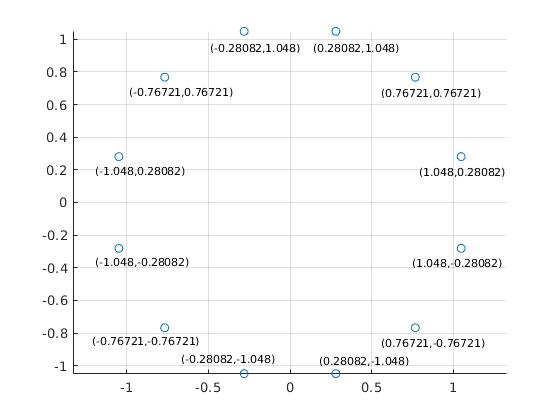
\includegraphics[scale = 0.7]{RootPlot2.jpg}
    \caption{Poles of Magnitude Plot of Analog LPF}
\end{figure}
Note that the above figure shows the poles of the Magnitude Plot of the Transfer Function. In order to get a stable Analog LPF, we must include the poles lying in the Left Half Plane in the Transfer Function(The poles are symmetric about origin and we can pick one from each pair to be a part of our Transfer Function).
\begin{equation*}
p_{1} = -0.2808 - 1.0480\iota
\end{equation*}
\begin{equation*}
p_{2} = -0.7672 - 0.7672\iota
\end{equation*}
\begin{equation*}
p_{3} = -1.0480 - 0.2808\iota
\end{equation*}
\begin{equation*}
p_{4} =-1.0480 + 0.2808\iota
\end{equation*}
\begin{equation*}
p_{5} = -0.7672  + 0.7672\iota
\end{equation*}
\begin{equation*}
p_{6} = -0.2808 + 1.0480\iota
\end{equation*}
\newpage
Using the above poles which are in the left half plane we can write the Analog Lowpass Transfer Function as:
\begin{equation*}
H_{analog,LPF}(s_{L}) = \frac{(\Omega _{c})^{N}}{(s_{L}-p_{1})(s_{L}-p_{2})(s_{L}-p_{3})(s_{L}-p_{4})(s_{L}-p_{5})(s_{L}-p_{6})}
\end{equation*}
\begin{equation*}
= \frac{1.6315}{(s_{L}^{2}+0.5616s_{L}+1.1772)(s_{L}^{2} + 1.5344s_{L} +1.1772)(s_{L}^{2}+2.0961s_{L}+1.1772)} 
\end{equation*}
\\%Note that the scaling of the numerator is done in order to obtain a DC gain of 1.
%--------------------------------------------------------------------------------------------------------------------------
\subsection{Analog Bandstop Transfer Function}
The transformation equation is given by:
\begin{equation*}
s_{L} = \frac{Bs}{\Omega _{0}^{2} + s^{2}}
\end{equation*}
Substituting the values of the parameters B(0.1325) and $\Omega _{0}$(0.2214), we get:
\begin{equation*}
s_{L} = \frac{0.1325s}{0.0490 + s^{2}}
\end{equation*}
Substituting this value into $H_{analog,LPF}(s_{L})$ we get $H_{analog,BSF}(s)$. It can be written in the form N(s)/D(s) where the coefficients of the polynomials N(s) and D(s) are given as:\\

\begin{table}[h!]
\centering
\begin{tabular}{|l|l|l|l|l|l|l|l|l|l|}\hline
Degree & $s^{12}$ & $s^{11}$ & $s^{10}$ & $s^{9}$ \\ \hline
Coefficient & 1($a_{12}$) & 0.4719($a_{11}$) & 0.4054($a_{10}$) & 0.1323($a_{9}$) \\\hline
\end{tabular}
%\caption{\label{tab:widgets}Coefficients of N(s)}
\end{table}
\begin{table}[h!]
\centering
\begin{tabular}{|l|l|l|l|l|l|l|l|l|l|}\hline
Degree & $s^{8}$ & $s^{7}$ & $s^{6}$ & $s^{5}$ \\ \hline
Coefficient & 0.0595($a_{8}$) & 0.01389($a_{7}$) & 0.004126($a_{6}$) & 0.00068($a_{5}$) \\\hline
\end{tabular}
%\caption{\label{tab:widgets}Coefficients of N(s)}
\end{table}
\begin{table}[h!]
\centering
\begin{tabular}{|l|l|l|l|l|l|l|l|l|l|}\hline
Degree & $s^{4}$ & $s^{3}$ & $s^{2}$ & $s^{1}$ & $s^{0}$ \\ \hline
Coefficient & 0.000143($a_{4}$) & 1.558*$10^{-5}$($a_{3}$) & 2.34*$10^{-6}$($a_{2}$) & 1.3348*$10^{-7}$($a_{1}$) & 1.386*$10^{-8}$($a_{0}$) \\\hline
\end{tabular}
\caption{\label{tab:widgets}Coefficients of D(s)}
\end{table}

\newpage
\begin{table}[h!]
\centering
\begin{tabular}{|l|l|l|l|l|l|l|l|l|l|}\hline
Degree & $s^{12}$ & $s^{10}$ & $s^{8}$ & $s^{6}$ \\ \hline
Coefficient & 1($b_{12}$) &  0.2941($b_{10}$) &  0.0360  ($b_{8}$)   & 0.024($b_{6}$) \\\hline
\end{tabular}
%\caption{\label{tab:widgets}Coefficients of N(s)}
\end{table}
\begin{table}[h!]
\centering
\begin{tabular}{|l|l|l|l|l|l|l|l|}\hline
Degree & $s^{4}$ &$s^{2}$ &$s^{0}$ \\ \hline
Coefficient &8.656*$10^{-5}$($b_{4}$)&  1.697*$10^{-6}$($b_{2}$)  & 1.3863*$10^{-8}$($b_{0}$)  \\\hline
\end{tabular}
\caption{\label{tab:widgets1}Coefficients of N(s)}
\end{table}
The coefficients of odd powers of s in N(s) are all 0.
\begin{comment}
\begin{equation*}
\frac{0.4333s^{4}}{(s^{8}+0.7341s^{7}+7.8768s^{6}+4.1873s^{5}+21.2172s^{4}+7.1529s^{3}+22.9855s^{2}+3.6592s^{1}+8.5154)}
\end{equation*}\\
\end{comment}
%--------------------------------------------------------------------------------------------------------------------------
\subsection{Discrete Time Filter Transfer Function}
To transform the analog domain transfer function into the discrete domain, we need to make use of the Bilinear Transformation which is given as:
\begin{equation*}
s = \frac{1-z^{-1}}{1+z^{-1}}
\end{equation*}
Using above equation we get $H_{discrete,BSF}(z)$ from  $H_{analog,BSF}(s)$.It can be written in the form N(z)/D(z) where the coefficients of the polynomials N(z) and D(z) are given as:\\
\begin{table}[h!]
\centering
\begin{tabular}{|l|l|l|l|l|l|l|l|l|l|}\hline
Degree & $z^{-12}$ & $z^{-11}$ & $z^{-10}$ & $z^{-9}$ \\ \hline
Coefficient &  0.64 ($b_{-12}$) &-6.94($b_{-11}$) & 35.3($b_{-10}$) &-110.79($b_{-9}$) \\\hline
\end{tabular}
%\caption{\label{tab:widgets}Coefficients of N(s)}
\end{table}
\begin{table}[h!]
\centering
\begin{tabular}{|l|l|l|l|l|l|l|l|l|l|}\hline
Degree & $z^{-8}$ & $z^{-7}$ & $z^{-6}$ & $z^{-5}$ \\ \hline
Coefficient & 238.9 ($b_{-8}$) & -372.68($b_{-7}$) &  431.15($b_{-6}$) &-372.68($b_{-5}$) \\\hline
\end{tabular}
%\caption{\label{tab:widgets}Coefficients of N(s)}
\end{table}
\begin{table}[h!]
\centering
\begin{tabular}{|l|l|l|l|l|l|l|l|l|l|}\hline
Degree & $z^{-4}$ & $z^{-3}$ & $z^{-2}$ & $z^{-1}$& $z^{0}$ \\ \hline
Coefficient & 238.9($b_{-4}$) &   -110.79($b_{-3}$) &  35.3($b_{-2}$) & -6.94($b_{-1}$) & 0.64($b_{0}$) \\\hline
\end{tabular}
\caption{\label{tab:widgets}Coefficients of N(z)}
\end{table}

%\vspace{1 cm}
\newpage

\begin{table}[h!]
\centering
\begin{tabular}{|l|l|l|l|l|l|l|l|l|l|}\hline
Degree & $z^{-12}$ & $z^{-11}$ & $z^{-10}$ & $z^{-9}$ \\ \hline
Coefficient &  0.41($a_{-12}$) &  -4.76($a_{-11}$) &  26.03($a_{-10}$) & -87.86($a_{-9}$) \\\hline
\end{tabular}
%\caption{\label{tab:widgets}Coefficients of N(s)}
\end{table}
\begin{table}[h!]
\centering
\begin{tabular}{|l|l|l|l|l|l|l|l|l|l|}
\hline
Degree & $z^{-8}$ & $z^{-7}$ & $z^{-6}$ & $z^{-5}$ \\ \hline
Coefficient & 203.91($a_{-8}$) & -342.53($a_{-7}$) &  426.97($a_{-6}$) &  -397.89($a_{-5}$) \\\hline
\end{tabular}
%\caption{\label{tab:widgets}Coefficients of N(s)}
\end{table}
\begin{table}[h!]
\centering
\begin{tabular}{|l|l|l|l|l|l|l|l|l|l|}
\hline
Degree & $z^{-4}$ & $z^{-3}$ & $z^{-2}$ & $z^{-1}$& $z^{0}$ \\ \hline
Coefficient & 275.14($a_{-4}$) &  -137.71($a_{-3}$) & 47.38($a_{-2}$) &  -10.07($a_{-1}$) & 1($a_{0}$) \\\hline
\end{tabular}
\caption{\label{tab:widgets}Coefficients of D(z)}
\end{table}

\begin{comment}
\begin{equation*}
\frac{0.0056-0.0224z^{-2}+0.0336z^{-4}-0.0224z^{-6}+0.0056z^{-8}}{1.0000+1.8627z^{-1}+4.4465z^{-2}+4.9605z^{-3}+6.2688z^{-4}+4.3615z^{-5}+3.4423z^{-6}+1.2554z^{-7}+0.5931z^{-8}}
\end{equation*}
\end{comment}
\begin{figure}[h!]
	\centering	
	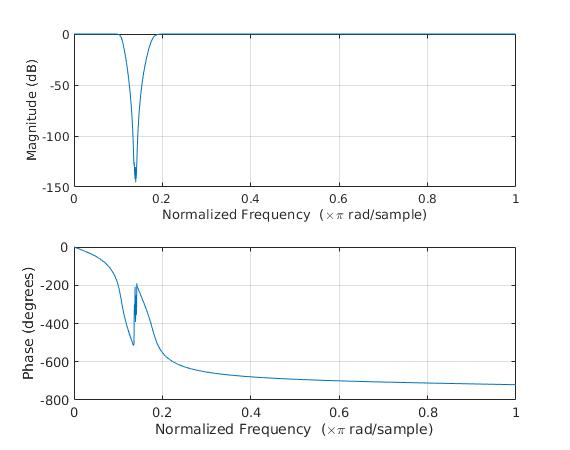
\includegraphics[width = 0.8\textwidth]{matlab_filter2.jpg}
    \caption{Plotting frequency and phase response of filter using freqz command of MATLAB}
\end{figure}
\newpage
%--------------------------------------------------------------------------------------------------------------------------
\newpage
\subsection{Realization using Direct Form \Rmnum{2}}
\begin{figure}[h!]
	\centering	
	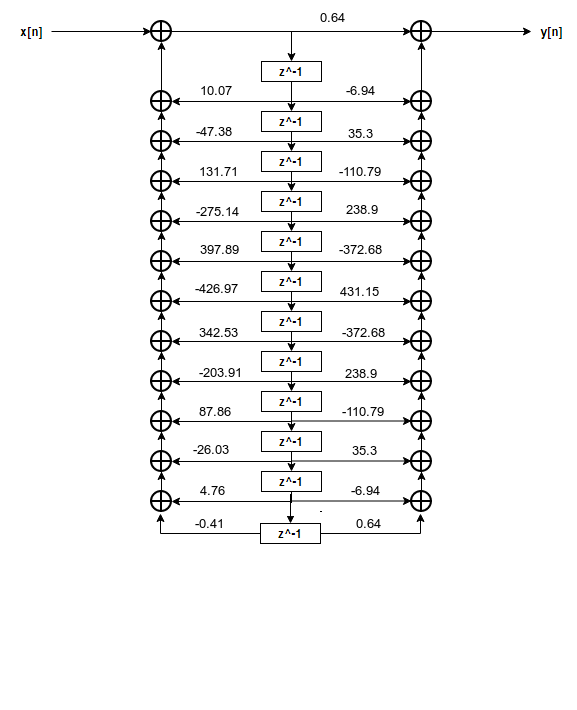
\includegraphics[scale = 0.6]{Butterworth_DirectForm_2.png}
    \caption{Direct Form \Rmnum{2} Block Diagram for $H_{discrete,BSF}(z)$}
\end{figure}

The negative of the denominator coefficients appear as gains on the side of the input sequence x[n] while the numerator coefficients appear on the side of the output y[n] as gains in the signal-flow graph representation of the Direct Form \Rmnum{2}.  
%--------------------------------------------------------------------------------------------------------------------------
\subsection{FIR Filter Transfer Function using Kaiser Window}
The tolerance in both the stopband and passband is given to be 0.15.\\
Therefore $\delta$ = 0.15 and we get the  minimum stopband attenuation to be:
\begin{equation*}
A = -20\log (0.15) = 16.4782 dB
\end{equation*}
Since A $<$ 21, we get $\beta$ to be 0 where  $\beta$ is the shape parameter of Kaiser window.\\
Now to estimate the window length required, we use the empirical formula for the lower bound on the window length.
\begin{equation*}
N \geq \frac{A-7.95}{2.285*\Delta\omega _{T}}
\end{equation*}
Here $\Delta\omega _{T}$ is the minimum transition width. In our case, the transition width is the same on either side of the passband. 
\begin{equation*}
\Delta\omega _{T} = \frac{2 kHz * 2\pi}{250 kHz} =  0.016\pi
\end{equation*}
\begin{equation*}
\therefore N \geq 74
\end{equation*}
The above equation gives a loose bound on the window length when the tolerance is not very stringent. On successive trials in MATLAB,it was found that a window length of \textbf{99} is required to satisfy the required constraints. Also, since $\beta$ is 0, the window is actually a rectangular window.\\
\\The time domain coefficients were obtained by first generating the ideal impulse response samples for the same length as that of the window. The Kaiser Window was generated using the MATLAB function and applied on the ideal impulse response samples. The band-stop impulse response samples were generated as the difference between three low-pass filters( all-pass - bandpass ) as done in class.
\newpage
\begin{figure}[h!]
	\centering
    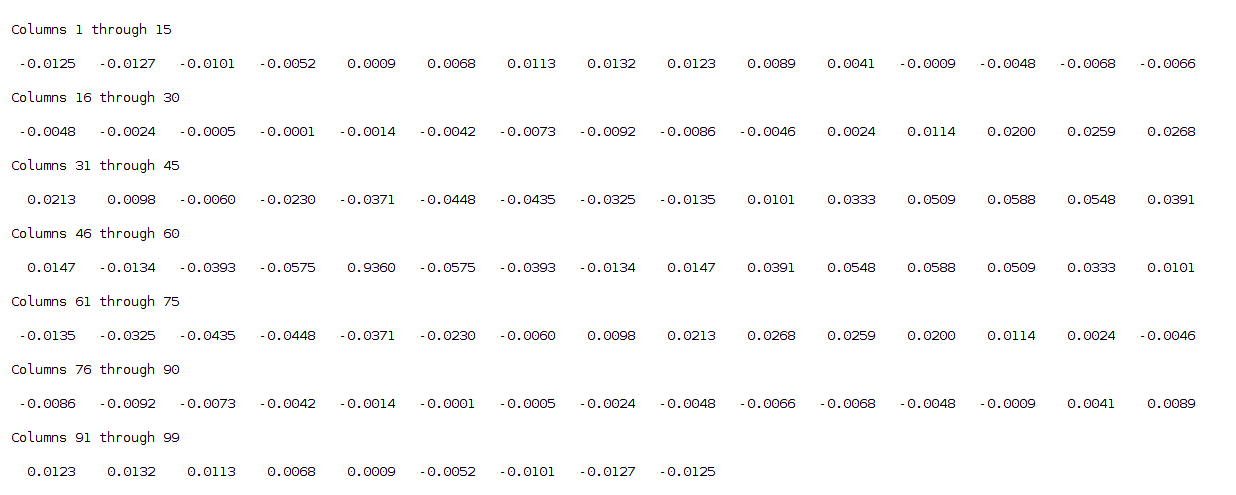
\includegraphics[width = 1\textwidth]{2firt.png}
    \caption{Time domain sequence values}
\end{figure}
The z-transform can simply be read off from the sequence values since its finite sequence.
\begin{figure}[h!]
	\centering
    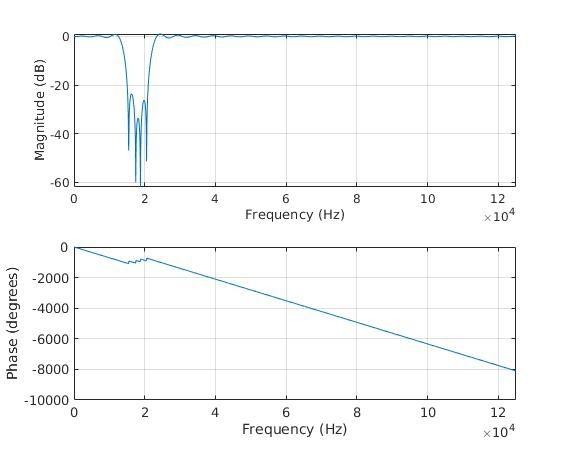
\includegraphics[width = 0.8\textwidth]{2fir.jpg}
    \caption{Plotting frequency and phase response of filter using freqz command of MATLAB}
\end{figure}
%--------------------------------------------------------------------------------------------------------------------------
%--------------------------------------------------------------------------------------------------------------------------
%--------------------------------------------------------------------------------------------------------------------------
\newpage
\section{MATLAB Plots}
\subsection{Filter 1 - Bandpass}
\subsubsection{IIR Filter}
\begin{figure}[h!]
	\centering	
	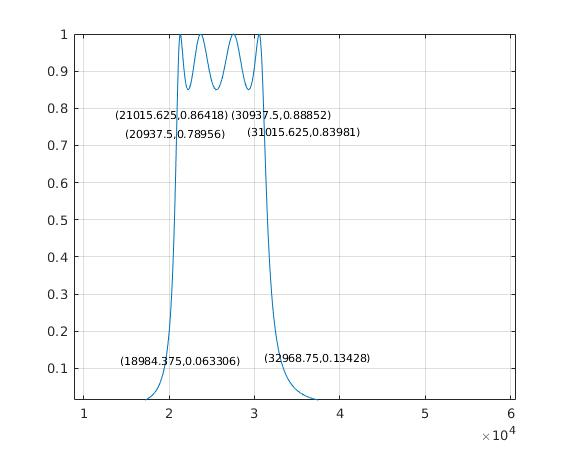
\includegraphics[width = 0.5\textwidth]{1fil.jpg}
    \caption{Frequency Response}
\end{figure}
From the above plot, I have verified that the passband tolerance and stopband attenuation have been satisfied. 
\begin{figure}[h!]
	\centering	
	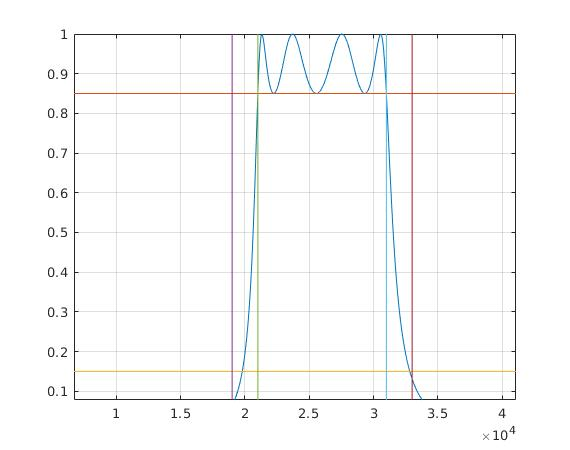
\includegraphics[width = 0.5\textwidth]{1filb.jpg}
    \caption{Frequency Response with boundaries}
\end{figure}
In the above plot, the band edge frequencies have been marked. From the magnitude at these frequencies it can be seen that the specifications required in the passband  and the stopband have been met.
\begin{figure}[h!]
	\centering	
	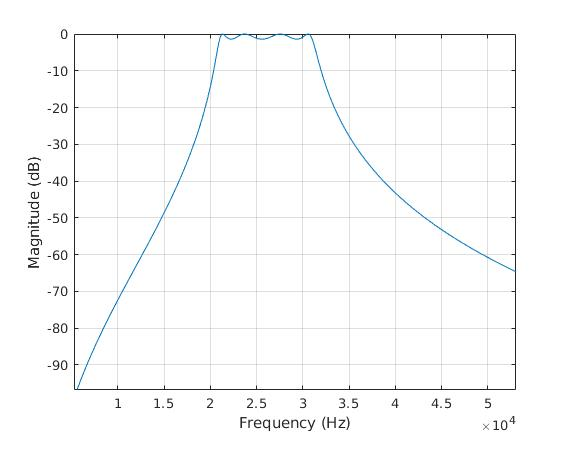
\includegraphics[width = 0.5\textwidth]{1filp.jpg}
    \caption{Frequency Response (in dB)}
\end{figure}
\begin{figure}[h!]
	\centering	
	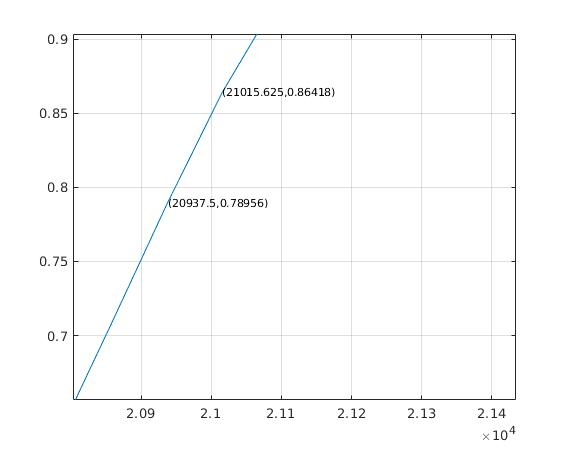
\includegraphics[width = 0.5\textwidth]{1pb1.jpg}
    \caption{Frequency Response- Around Passband Limit 1}
\end{figure}
\begin{figure}[h!]
	\centering	
	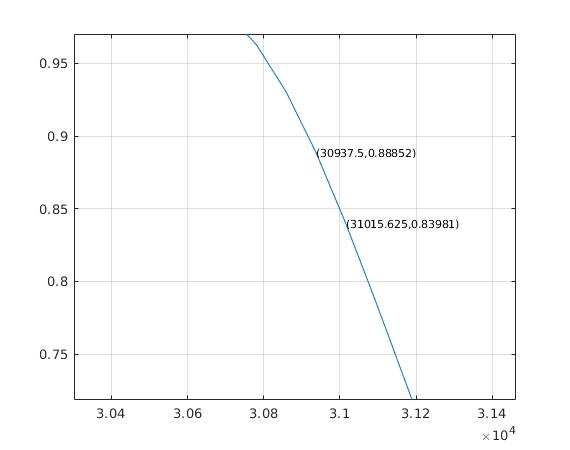
\includegraphics[width = 0.5\textwidth]{1pb2.jpg}
    \caption{Frequency Response- Around Passband Limit 2}
\end{figure}
\begin{figure}[h!]
	\centering	
	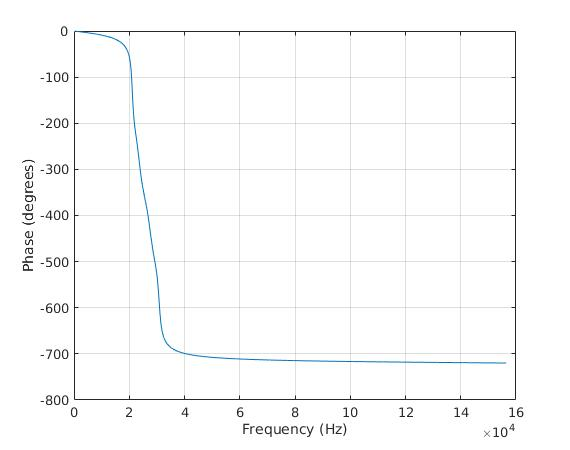
\includegraphics[width = 0.5\textwidth]{1ph.jpg}
    \caption{Phase Response}
\end{figure}
\newpage
It can be seen that the \textbf{phase response} is \textbf{not linear}.
\begin{figure}[h!]
	\centering	
	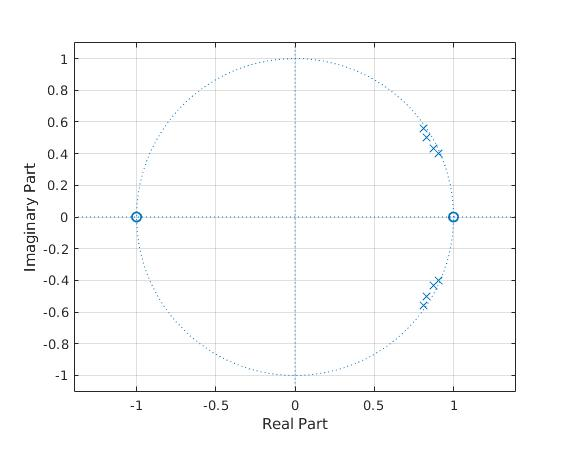
\includegraphics[width = 0.5\textwidth]{1pz.jpg}
    \caption{Pole-Zero map (all poles within unit circle, hence stable)}
\end{figure}
\newpage
\
\newpage
\subsubsection{FIR Filter}
\begin{figure}[h!]
	\centering	
	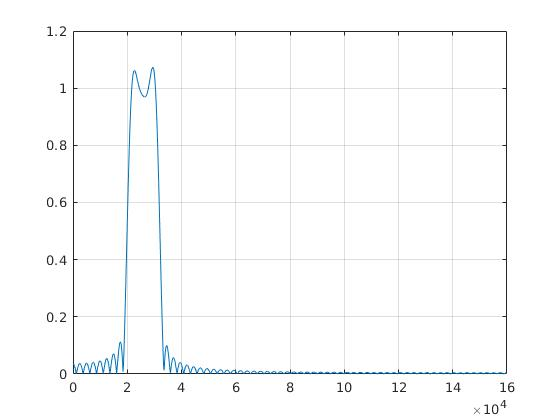
\includegraphics[width = 0.6\textwidth]{1firm.jpg}
    \caption{Frequency Response}
\end{figure}
From the above plot, I have verified that the passband tolerance and stopband attenuation have been satisfied. It can be seen that the FIR Filter is indeed giving us a \textbf{Linear Phase} response which is desired.
\begin{figure}[h!]
	\centering	
	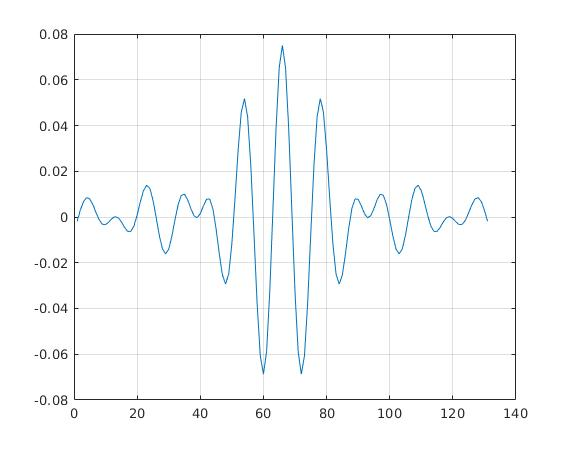
\includegraphics[width = 0.5\textwidth]{1firc.jpg}
    \caption{Time Domain Sequence}
\end{figure}
\newpage
\begin{figure}[h!]
	\centering	
	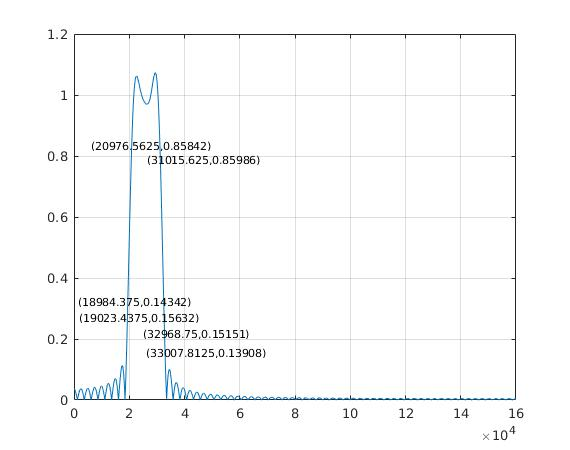
\includegraphics[width = 0.6\textwidth]{1firb.jpg}
    \caption{Magnitude Plot}
\end{figure}
In the above plot, the band edge frequencies have been marked. From the magnitude at these frequencies it can be seen that the specifications required in the passband and the stopband have been met.
\begin{figure}[h!]
	\centering	
	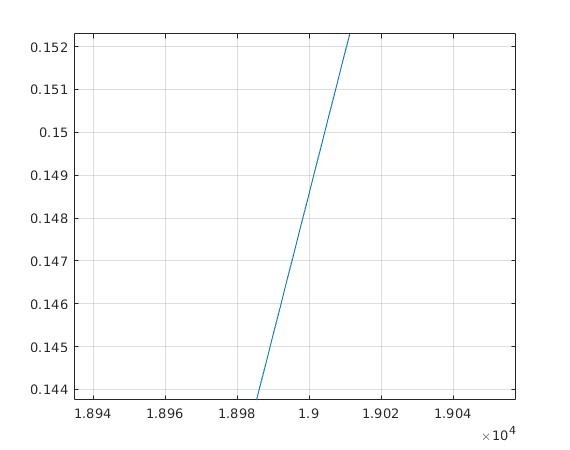
\includegraphics[width = 0.5\textwidth]{1firsb1.jpg}
    \caption{Frequency Response- Around Stopband Limit 1}
\end{figure}
\begin{figure}[h!]
	\centering	
	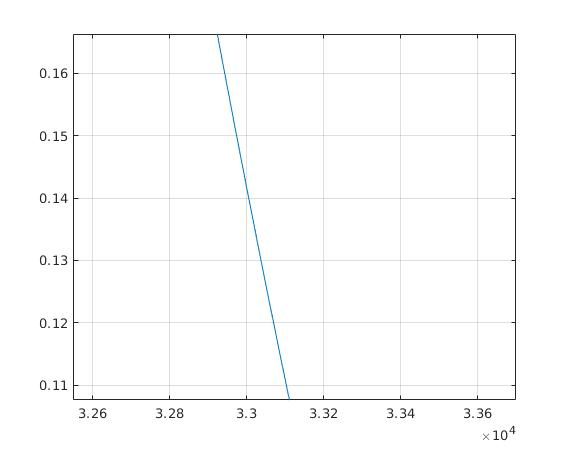
\includegraphics[width = 0.5\textwidth]{1firsb2.jpg}
    \caption{Frequency Response- Around Stopband Limit 2}
\end{figure}
\clearpage
\newpage
\subsection{Filter 2 - Bandstop}
\subsubsection{IIR Filter}
\begin{figure}[h!]
	\centering	
	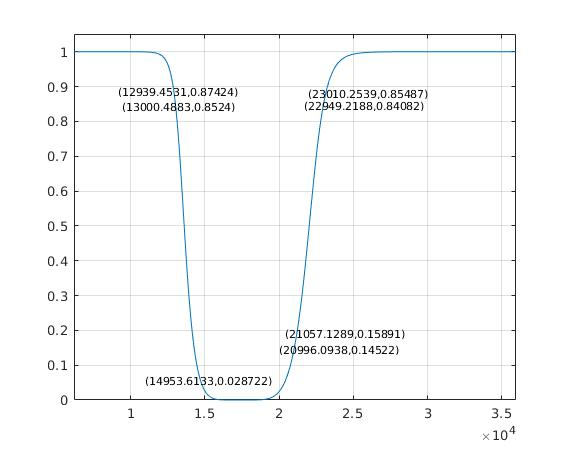
\includegraphics[width = 0.5\textwidth]{2fil.jpg}
    \caption{Frequency Response}
\end{figure}
From the above plot, I have verified that the passband tolerance and stopband attenuation have been satisfied. 
\begin{figure}[h!]
	\centering	
	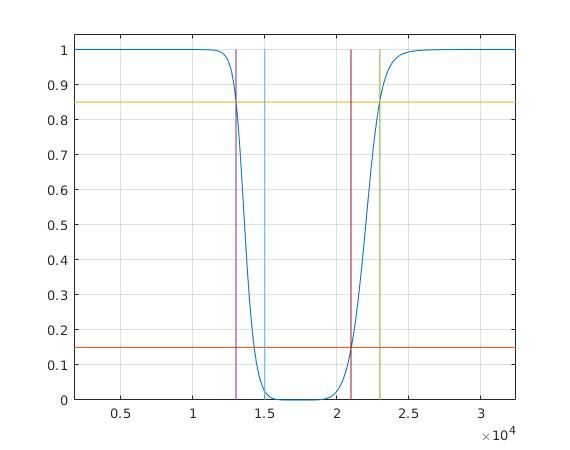
\includegraphics[width = 0.5\textwidth]{2filb.jpg}
    \caption{Frequency Response with boundaries}
\end{figure}
In the above plot, the band edge frequencies have been marked. From the magnitude at these frequencies it can be seen that the specifications required in the passband  and the stopband have been met.
\begin{figure}[h!]
	\centering	
	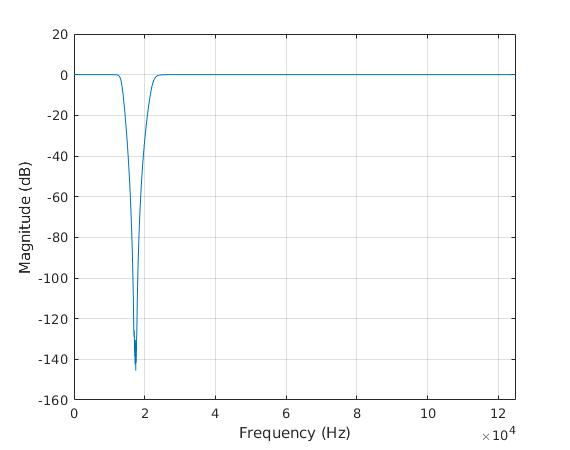
\includegraphics[width = 0.5\textwidth]{2filp.jpg}
    \caption{Frequency Response (in dB)}
\end{figure}
\begin{figure}[h!]
	\centering	
	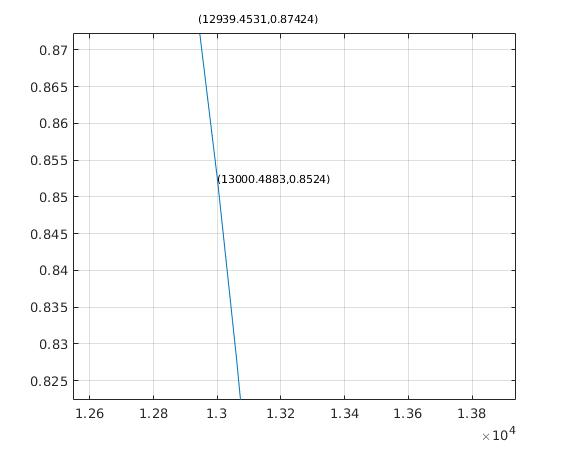
\includegraphics[width = 0.5\textwidth]{2pb1.jpg}
    \caption{Frequency Response- Around Passband Limit 1}
\end{figure}
\clearpage
\begin{figure}[h!]
	\centering	
	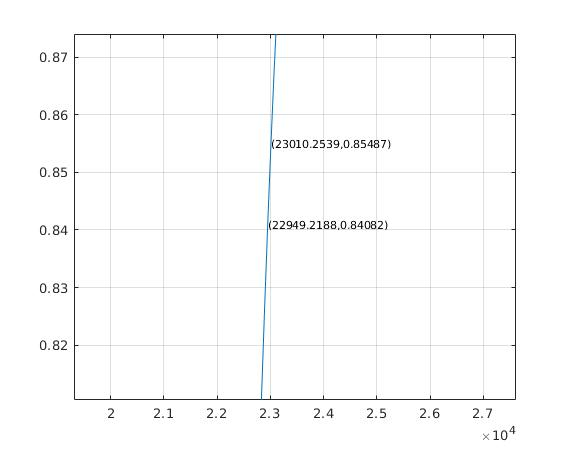
\includegraphics[width = 0.5\textwidth]{2pb2.jpg}
    \caption{Frequency Response- Around Passband Limit 2}
\end{figure}
\begin{figure}[h!]
	\centering	
	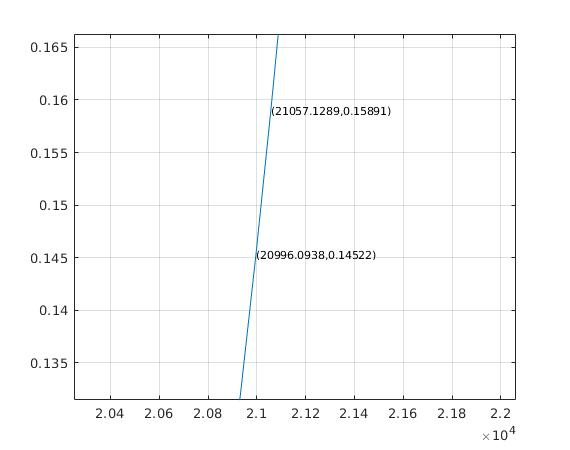
\includegraphics[width = 0.5\textwidth]{2sb2.jpg}
    \caption{Frequency Response- Around Stopband Limit 2}
\end{figure}
\clearpage
\begin{figure}[h!]
	\centering	
	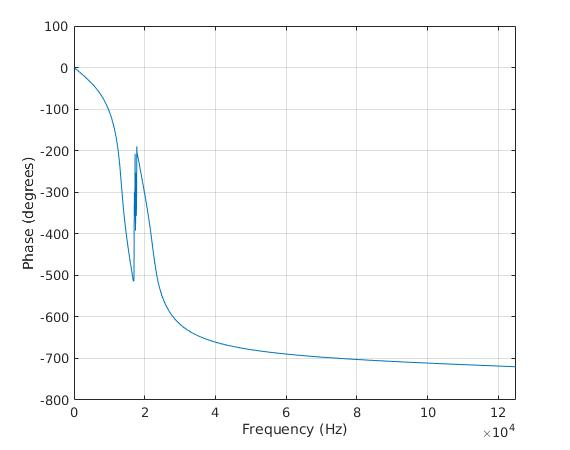
\includegraphics[width = 0.5\textwidth]{2ph.jpg}
    \caption{Phase Response}
\end{figure}
It can be seen that the \textbf{phase response} is \textbf{not linear}.

\begin{figure}[h!]
	\centering	
	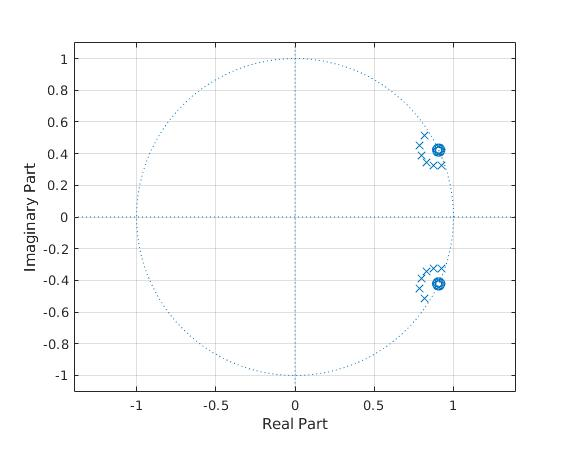
\includegraphics[width = 0.5\textwidth]{2pz.jpg}
    \caption{Pole-Zero map (all poles within unit circle, hence stable)}
\end{figure}\newpage
\subsubsection{FIR Filter}
\begin{figure}[h!]
	\centering	
	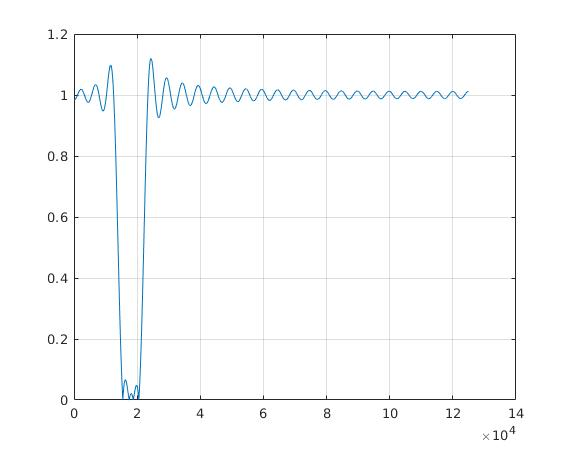
\includegraphics[width = 0.6\textwidth]{2firm.jpg}
    \caption{Frequency Response}
\end{figure}
From the above plot, I have verified that the passband tolerance and stopband attenuation have been satisfied. It can be seen that the FIR Filter indeed gives us a \textbf{Linear Phase} response which is desired.
\begin{figure}[h!]
	\centering	
	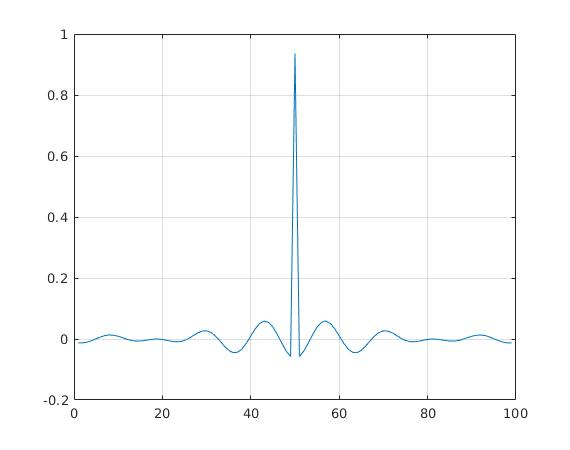
\includegraphics[width = 0.5\textwidth]{2firc.jpg}
    \caption{Time Domain Sequence}
\end{figure}
\newpage
\begin{figure}[h!]
	\centering	
	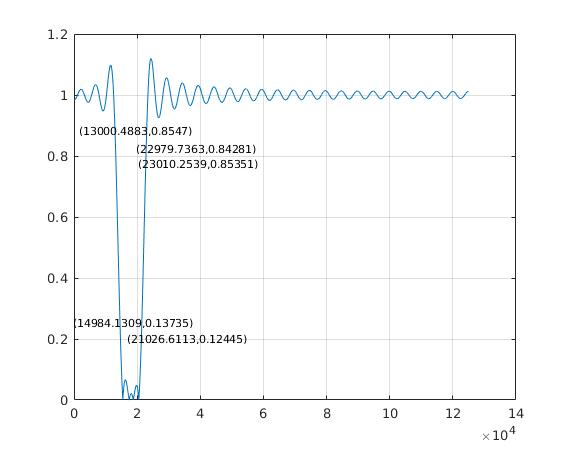
\includegraphics[width = 0.6\textwidth]{2firb.jpg}
    \caption{Magnitude Plot}
\end{figure}
In the above plot, the band edge frequencies have been marked. From the magnitude at these frequencies it can be seen that the specifications required in the passband and the stopband have been met.
\begin{figure}[h!]
	\centering	
	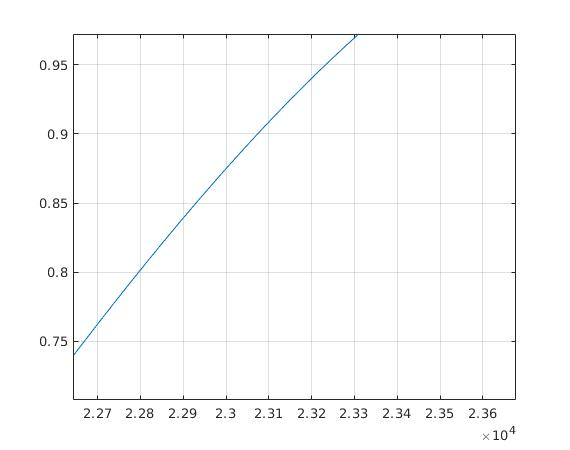
\includegraphics[width = 0.5\textwidth]{2firpb2.jpg}
    \caption{Frequency Response- Around Passband Limit 2}
\end{figure}
\end{document}